\documentclass{beamer}

\usepackage{minted}
\setminted{breaklines,python3=true}
\newminted{python}{}
\newminted{pycon}{}
\newcommand{\codepause}{\pause\vspace{-6pt}}

\usepackage{graphicx}


\begin{document}

\begin{frame}
  \frametitle{Why Python?}
  \begin{itemize}
    \pause
  \item Due to its simple syntax and dynamic typing, Python is easy to learn.
    \pause
  \item Python is widely used in academia and industry for numerical and scientific computing (deep learning is especially hot right now).
    \pause
  \item Unlike MATLAB, Python is a general-purpose language, so it has wide applicability even outside those fields (there's a Python library for everything).
    \pause
  \item Python is open-source.
  \end{itemize}
\end{frame}

\begin{frame}
  \frametitle{CoCalc}
  We will be using an interactive Web-based interface called CoCalc. This requires signup.
  \begin{enumerate}
  \item Go to https://cocalc.com/. Click ``Create Account!'' and enter your information. Create an account.
  \item Now we are at the ``Projects'' screen. In the textbox that says ``Project title'', enter a title -- something like ``First Day Tutorial'' -- and click ``Create Project''. Then click on your new project.
  \item On the bar along the top, click the arrow next to ``New'' and select ``Jupyter Notebook (.ipynb)''. You can call it whatever you want. Select the Python 3 kernel.
  \end{enumerate}
  Now we can start entering Python code. Press Ctrl+Enter in a cell to execute it.
\end{frame}

\begin{frame}[fragile]
  \frametitle{\texttt{'Hello, world!'}; Strings}
  \inputminted[firstline=1,lastline=2]{pycon}{code/hello_world.txt}
  \codepause
  \inputminted[firstline=3,lastline=4]{pycon}{code/hello_world.txt}
  \codepause
  \inputminted[firstline=5,lastline=6]{pycon}{code/hello_world.txt}
  \codepause
  \inputminted[firstline=7,lastline=8]{pycon}{code/hello_world.txt}
\end{frame}

\begin{frame}[fragile]
  \frametitle{Basic Arithmetic; Order of Operations}
  \inputminted[firstline=1,lastline=4]{pycon}{code/order_of_operations.txt}
  \codepause
  \inputminted[firstline=5,lastline=8]{pycon}{code/order_of_operations.txt}
  \codepause
\inputminted[firstline=9,lastline=12]{pycon}{code/order_of_operations.txt}
\end{frame}

\begin{frame}[fragile]
  \frametitle{Comparisons}
  \inputminted[firstline=1,lastline=4]{pycon}{code/comparisons.txt}
  \codepause
  \inputminted[firstline=5,lastline=6]{pycon}{code/comparisons.txt}
  \codepause
  \inputminted[firstline=7,lastline=10]{pycon}{code/comparisons.txt}
\end{frame}

\begin{frame}[fragile]
  \frametitle{Booleans}
  \inputminted[firstline=1,lastline=2]{pycon}{code/booleans.txt}
  \codepause
  \inputminted[firstline=3,lastline=4]{pycon}{code/booleans.txt}
  \codepause
  \inputminted[firstline=5,lastline=6]{pycon}{code/booleans.txt}
  \codepause
  \inputminted[firstline=7,lastline=8]{pycon}{code/booleans.txt}
\end{frame}

\begin{frame}[fragile]
  \frametitle{Short-Circuiting (and Division by Zero)}
  \inputminted[firstline=1,lastline=2]{pycon}{code/short_circuit.txt}
  \codepause
  \inputminted[firstline=3,lastline=6]{pycon}{code/short_circuit.txt}
  \codepause
  \inputminted[firstline=7,lastline=8]{pycon}{code/short_circuit.txt}
  \codepause
  \inputminted[firstline=9,lastline=12]{pycon}{code/short_circuit.txt}
\end{frame}

\begin{frame}[fragile]
  \frametitle{Modulo}
\begin{pyconcode}
>>> 5 % 5
0
>>> 6 % 5
1
>>> 7 % 5
2
>>> 8 % 5
3
>>> 9 % 5
4
>>> 10 % 5
0
\end{pyconcode}
\end{frame}

\begin{frame}[fragile]
  \frametitle{Defining Functions}
  \inputminted[firstline=1,lastline=1]{python}{code/divides.txt}
  \codepause
  \inputminted[firstline=2,lastline=2]{python}{code/divides.txt}
\end{frame}

\begin{frame}[fragile]
  \frametitle{Calling Functions}
\begin{pyconcode}
>>> divides(2, 4)
True
>>> divides(3, 4)
False
\end{pyconcode}
\end{frame}

\begin{frame}[fragile]
  \frametitle{\texttt{if}/\texttt{elif}/\texttt{else}}
  \inputminted[firstline=1,lastline=1]{python}{code/sgn.txt}
  \codepause
  \inputminted[firstline=2,lastline=3]{python}{code/sgn.txt}
  \codepause
  \inputminted[firstline=4,lastline=5]{python}{code/sgn.txt}
  \codepause
  \inputminted[firstline=6,lastline=7]{python}{code/sgn.txt}
\end{frame}

\begin{frame}[fragile]
  \frametitle{While-loops (and variables)}
  \inputminted[firstline=1,lastline=1]{python}{code/is_prime.txt}
  \codepause
  \inputminted[firstline=2,lastline=2]{python}{code/is_prime.txt}
  \codepause
  \inputminted[firstline=3,lastline=3]{python}{code/is_prime.txt}
  \codepause
  \inputminted[firstline=4,lastline=5]{python}{code/is_prime.txt}
  \codepause
  \inputminted[firstline=6,lastline=6]{python}{code/is_prime.txt}
  \codepause
  \inputminted[firstline=7,lastline=7]{python}{code/is_prime.txt}
\end{frame}

\begin{frame}[fragile]
  \frametitle{For-loops}
\begin{pythoncode}
def is_prime_2(n):
    for i in range(2, n):
        if divides(i, n):
            return False
    return True
\end{pythoncode}
\end{frame}

\begin{frame}[fragile]
  \frametitle{\texttt{range}}
  \inputminted[firstline=1,lastline=2]{python}{code/range.txt}
  \codepause
  \inputminted[firstline=3,lastline=4]{python}{code/range.txt}
  \codepause
  \inputminted[firstline=5,lastline=6]{python}{code/range.txt}
\end{frame}

\begin{frame}[fragile]
  \frametitle{Lists}
  \inputminted[firstline=1,lastline=1]{python}{code/lists.txt}
  \codepause
  \inputminted[firstline=2,lastline=3]{python}{code/lists.txt}
  \codepause
  \inputminted[firstline=4,lastline=4]{python}{code/lists.txt}
  \codepause
  \inputminted[firstline=5,lastline=6]{python}{code/lists.txt}
  \codepause
  \inputminted[firstline=7,lastline=8]{python}{code/lists.txt}
  \codepause
  \inputminted[firstline=9,lastline=10]{python}{code/lists.txt}
  \codepause
  \inputminted[firstline=11,lastline=12]{python}{code/lists.txt}
\end{frame}

\begin{frame}[fragile]
  \frametitle{Lists (and Dot-Syntax)}
  \inputminted[firstline=1,lastline=2]{pycon}{code/lists2.txt}
  \codepause
  \inputminted[firstline=3,lastline=4]{pycon}{code/lists2.txt}
  \codepause
  \inputminted[firstline=5,lastline=5]{pycon}{code/lists2.txt}
  \codepause
  \inputminted[firstline=6,lastline=7]{pycon}{code/lists2.txt}
  \codepause
  \inputminted[firstline=8,lastline=8]{pycon}{code/lists2.txt}
  \codepause
  \inputminted[firstline=9,lastline=10]{pycon}{code/lists2.txt}
  \codepause
  \inputminted[firstline=11,lastline=12]{pycon}{code/lists2.txt}
\end{frame}

\begin{frame}[fragile]
  \frametitle{Assignment}
  \inputminted[firstline=1,lastline=2]{pycon}{code/assignment.txt}
  \codepause
  \inputminted[firstline=3,lastline=3]{pycon}{code/assignment.txt}
  \codepause
  \inputminted[firstline=4,lastline=5]{pycon}{code/assignment.txt}
  \codepause
  \inputminted[firstline=6,lastline=6]{pycon}{code/assignment.txt}
  \codepause
  \inputminted[firstline=7,lastline=8]{pycon}{code/assignment.txt}
  \codepause
  \inputminted[firstline=9,lastline=9]{pycon}{code/assignment.txt}
  \codepause
  \inputminted[firstline=10,lastline=10]{pycon}{code/assignment.txt}
\end{frame}

\begin{frame}[fragile]
  \frametitle{Slicing}
  \inputminted[firstline=1,lastline=3]{pycon}{code/slicing.txt}
  \codepause
  \inputminted[firstline=4,lastline=5]{pycon}{code/slicing.txt}
  \codepause
  \inputminted[firstline=6,lastline=7]{pycon}{code/slicing.txt}
  \codepause
  \inputminted[firstline=8,lastline=9]{pycon}{code/slicing.txt}
  \codepause
  \inputminted[firstline=10,lastline=11]{pycon}{code/slicing.txt}
  \codepause
  \inputminted[firstline=12,lastline=13]{pycon}{code/slicing.txt}
\end{frame}


\begin{frame}[fragile]
  \frametitle{Tuples}
  \inputminted[firstline=1,lastline=1]{pycon}{code/tuples.txt}
  \codepause
  \inputminted[firstline=2,lastline=3]{pycon}{code/tuples.txt}
  \codepause
  \inputminted[firstline=4,lastline=5]{pycon}{code/tuples.txt}
  \codepause
  \inputminted[firstline=6,lastline=9]{pycon}{code/tuples.txt}
  \codepause
  \inputminted[firstline=10,lastline=13]{pycon}{code/tuples.txt}
\end{frame}

\begin{frame}[fragile]
  \frametitle{Tuples}
  \inputminted[firstline=14,lastline=14]{pycon}{code/tuples.txt}
  \codepause
  \inputminted[firstline=15,lastline=16]{pycon}{code/tuples.txt}
  \codepause
  \inputminted[firstline=17,lastline=18]{pycon}{code/tuples.txt}
  \codepause
  \inputminted[firstline=19,lastline=19]{pycon}{code/tuples.txt}
  \codepause
  \inputminted[firstline=20,lastline=21]{pycon}{code/tuples.txt}
  \codepause
\end{frame}

\begin{frame}[fragile]
  \frametitle{Tuples}
  \inputminted[firstline=22,lastline=22]{pycon}{code/tuples.txt}
  \codepause
  \inputminted[firstline=23,lastline=24]{pycon}{code/tuples.txt}
  \codepause
  \inputminted[firstline=25,lastline=26]{pycon}{code/tuples.txt}
  \codepause
  \inputminted[firstline=27,lastline=28]{pycon}{code/tuples.txt}
  \codepause
  \inputminted[firstline=29,lastline=29]{pycon}{code/tuples.txt}
  \codepause
  \inputminted[firstline=30,lastline=31]{pycon}{code/tuples.txt}
  \codepause
  \inputminted[firstline=32,lastline=33]{pycon}{code/tuples.txt}
\end{frame}

% \begin{frame}[fragile]
%   \frametitle{An Algorithm}
% \begin{pythoncode}
% def factorize(n):
%     factors = []
%     i = 2
%     while i <= n:
%         if divides(i, n):
%             factors.append(i)
%             n /= i
%         else:
%             i += 1
%     return factors
% \end{pythoncode}
% \end{frame}

% \begin{frame}[fragile]
%   \frametitle{Imports}
% \begin{pythoncode}
% from collections import Counter

% def factorize(n):
%     factors = Counter()
%     i = 2
%     while i <= n:
%         if divides(i, n):
%             factors[i] += 1
%             n /= i
%         else:
%             i += 1
%     return factors
% \end{pythoncode}
% \end{frame}

\begin{frame}[fragile]
  \frametitle{Scatter Plots (and list-comprehensions)}
  \inputminted[firstline=1,lastline=1]{python}{code/scatter.txt}
  \codepause
  \inputminted[firstline=2,lastline=2]{python}{code/scatter.txt}
  \codepause
  \inputminted[firstline=3,lastline=3]{python}{code/scatter.txt}
  \codepause
  \inputminted[firstline=4,lastline=4]{python}{code/scatter.txt}
  \codepause
  \inputminted[firstline=5,lastline=5]{python}{code/scatter.txt}
\end{frame}

\begin{frame}
  \centerline{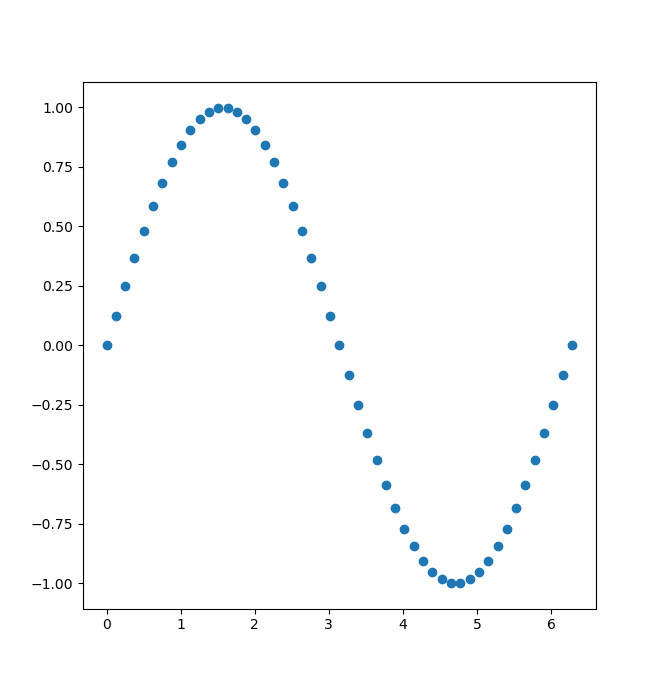
\includegraphics[scale=0.5]{image/scatter_sin.png}}
\end{frame}

\begin{frame}[fragile]
  \frametitle{Line Plots}
\begin{pyconcode}
>>> plt.plot(xs, ys)
\end{pyconcode}
\end{frame}

\begin{frame}
  \centerline{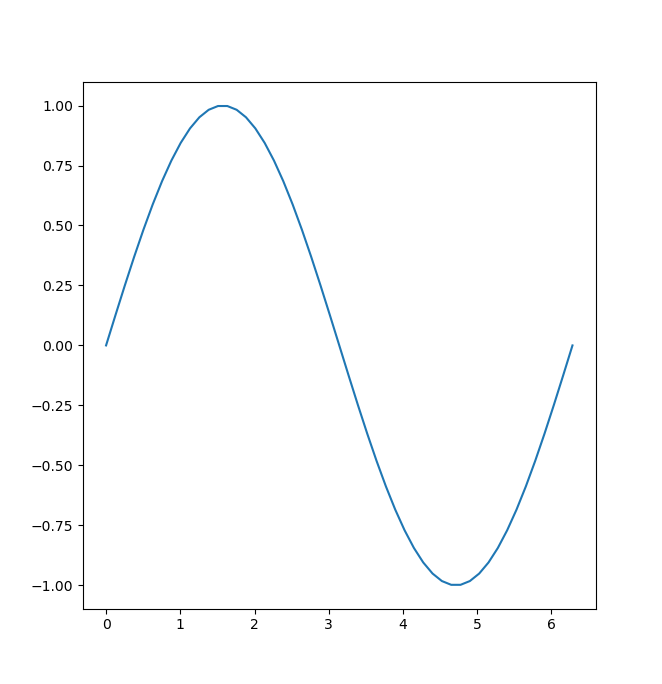
\includegraphics[scale=0.5]{image/plot_sin.png}}
\end{frame}

\end{document}

%%% Local Variables:
%%% TeX-command-extra-options: "-shell-escape"
%%% End:
